\chapter{Infraestrutura da rede de medidores}
\label{c:infraestrutura_da_rede_de_medidores}
% ---
A infraestrutura da rede de medidores da Universidade Federal de Goiás foi montada com o intuito de permitir realizar o monitoramento do consumo energético em vários níveis, desde uma medição geral, de maneira semelhante ao que é feito pela concessionária de energia, passando por uma medição em cada QDC de cada prédio, até a medição de um equipamento em específico, por exemplo o sistema de ar condicionado de um centro de aulas. Além disso essa infraestrutura deve contemplar o monitoramento da Potência Gerada pela planta fotovoltaica dos \textit{campus}.

Cada medidor em cada um desses pontos é um escravo da rede \textit{Modbus} de medição e possui um identificador próprio que o separa dos demais, portanto deve-se também ter um mestre para gerenciar essa estrutura, permitindo requisitar os dados de medição, cadastrar novos medidores, alterar endereçamento IP, identificar o status atual de cada medidor.

Abaixo, será descrito cada ponto de medição e após isso, será exposto um visual esquemático geral dessa rede onde cada ponto terá uma representatividade, demonstrando como cada comunicação em particular forma a infraestrutura completa da rede de medidores. Todos os dispositivos utilizados para compor a rede de medição são da marca CCK, incluindo o \textit{software} de monitoramento que cria o mestre da rede e permite o gerenciamento dos escravos.

\section{Medição de Fronteira}
\label{sec:medicao-de-fronteira}

Na medição de fronteira, é instalado o dispositivo CCK 6700E que é responsável por fazer a medição das fases, onde através de uma tomada de isolação ótica CCK 50, ele se conecta ao medidor da concessionária fazendo assim a leitura dos dados e armazenando em uma memória de massa que suporta um período de 35 dias, sobrescrevendo o primeiro dia após a inserção do trigésimo sexto. Abaixo, uma representação desse sistema de medição.

\begin{figure}[H]
    \centering
    \caption{Esquema Conexões Medição de Fronteira}
    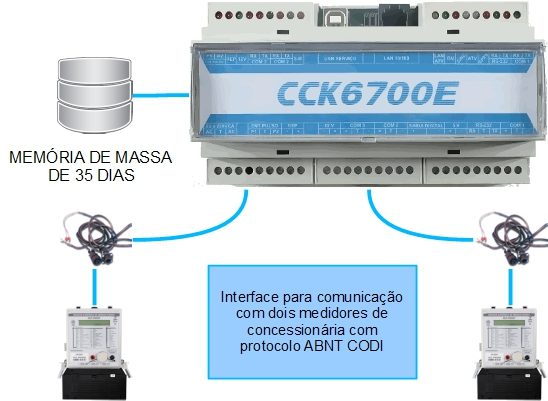
\includegraphics[width=0.8\linewidth]{imagens/cck6700e-esquema.jpg}
    \caption*{Fonte: \citeonline{cck6700E}}
    \label{fig:my_label}
\end{figure}

Feita essa comunicação com medidor, a comunicação do CCK 6700E com o mestre pode ser feito por:
\begin{itemize}
    \item Cabo UTP - É feita a conexão direta entre o dispositivo e o \textit{Switch} com a porta configurada para a VLAN da rede \textit{Modbus}
    \item Fibra Ótica - Através de um conversor de mídia o medidor é conectado à rede por fibra ótica onde na outra extremidade é usado outro conversor para receber a fibra e converter para UTP novamente
    \item Comunicação por Rádio - Um dispositivo recebe os sinais dos medidores através do protocolo RS485, enviando os dados por rádio frequência até outro dispositivo que recebe esse sinal e envia para um dispositivo CCK 7010W que faz a conversão de comunicação serial para Ethernet.
\end{itemize}

\section{Medição Interna}

Cada medidor de fronteira das unidades consumidoras fornece energia para um ou mais prédios de determinada região, sendo assim para um monitoramento mais preciso, faz-se necessário a implantação de subsistemas de medição específicos para cada edificação ou até mesmo em cenários onde se quer ter um controle sobre um consumo mais específico, pode-se ser instalado um medidor em um circuito mais fechado.

O dispositivo responsável por essa medição é o CCK 4400ME, fazendo a leitura e enviando através dos três modos citados na seção \ref{sec:medicao-de-fronteira}. Esse aparelho também possui memória de massa para armazenamento de até 35 dias de leitura.

Além da medição de prédios e equipamentos específicos, o CCK 4400ME é responsável por fazer a leitura de geração dos sistemas de placas fotovoltaicas dos blocos da Universidade. Essa medição é feita através de conexão com a saída do inversor do sistema gerador, enviando os dados para o mestre da rede através dos 3 tipos de comunicação disponíveis.

\section{Diagrama Esquemático Infraestrutura da Rede}

Descrito os modos de medição e comunicação dos diferentes pontos da rede, pode-se resumir todos os modos de conexão utilizados para os vários cenários da rede de medições através do diagrama esquemático abaixo:
\newline

\begin{figure}[H]
    \centering
    \caption{Diagrama Esquemático Rede Modbus de Monitoramento da Universidade Federal de Goiás}
    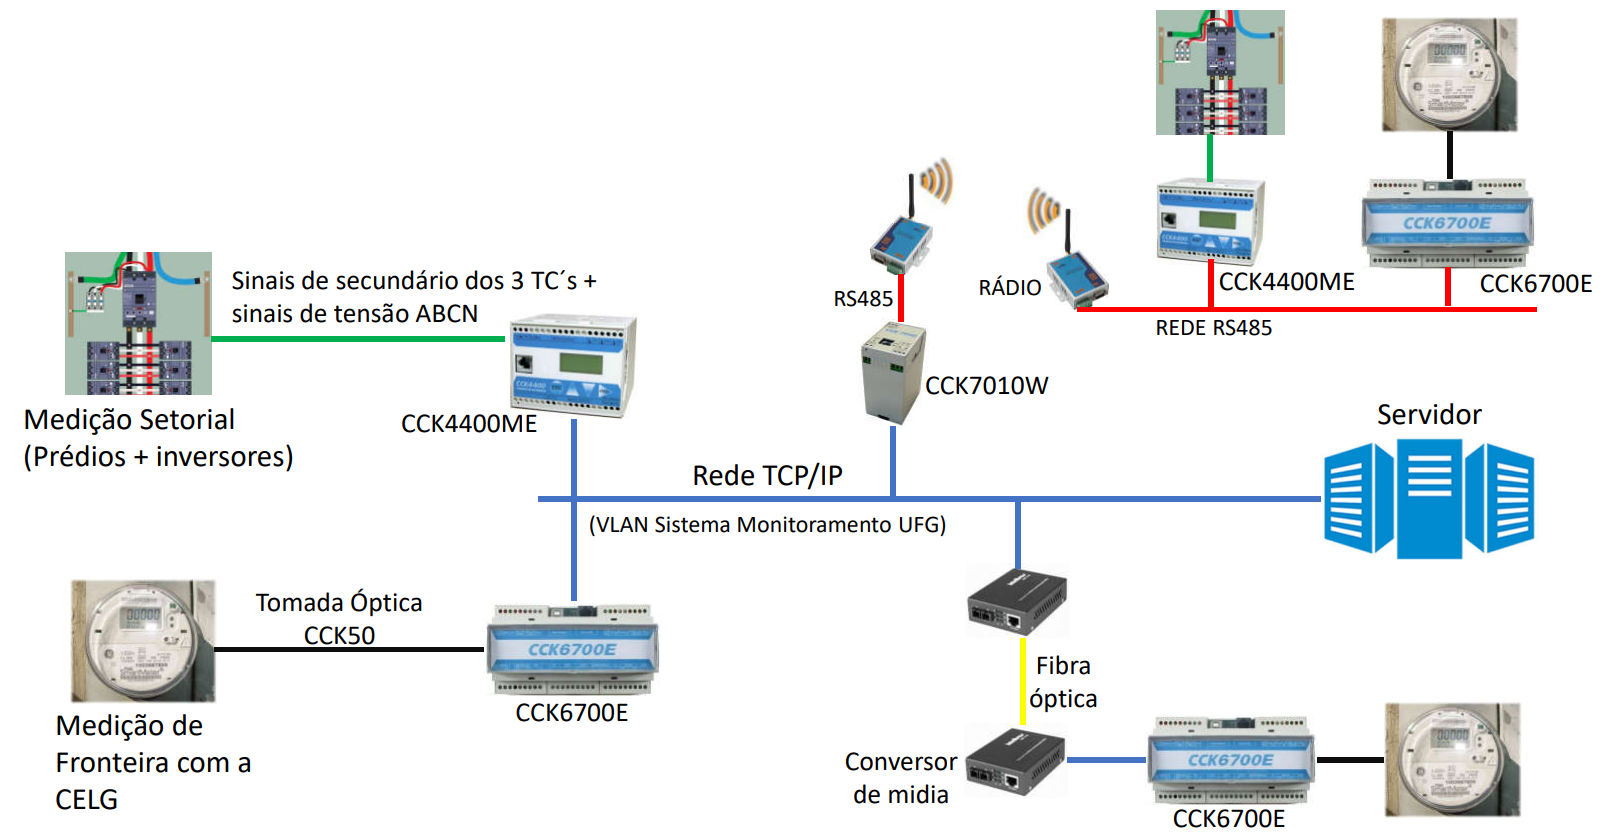
\includegraphics[width=\linewidth]{imagens/esquema-rede-modbus.png}
    \label{fig:diagrama-rede-ufg}
\end{figure}
